
\documentclass{report}
\usepackage{amssymb, amsmath}
\usepackage{graphicx}
\usepackage{float}

\title{Reporte Tarea 4}
\date{12 de Octubre de 2022}
\author{Nestor Adrian Sandoval Ortiz}

\begin{document}
    \maketitle

    \chapter{Funciones monovariables}
        \paragraph{Introduccion}
        A continuacion se presentan 5 funciones que serviran como punto de comparacion para 5 algoritmos de optimizacion sin restricciones.
        Es importante mencionar que, con el fin de mantener una condicion y/o cantidad de iteraciones justa, se ha planteado al numero "100"
        como parametro de "paro" en todas las funciones, es decir, en aquellas funciones que dependan de un determinado numero de iteraciones,
        estas sumaran 100, mientras que, en las que dependan de un valor concreto de "error", este mismo sera ubicado de tal forma que sus cantidades
        de iteraciones sean lo mas cercanas a 100
        Por ultimo, cabe destacar que se realizaran 1000 ejecuciones independientes de cada algoritmo, con el fin de conocer la media de sus valores
        asi como su mejor y peor desempeño.

        \pagebreak

        \section{Primera Funcion}
            \begin{equation*}
                f(x)=3x^4+(x-1)^2
            \end{equation*}

            \begin{figure}[H]
                \includegraphics[width=\linewidth]{/Users/lloydna/Desktop/UP/5° Semestre/Optimizacion/Optimizacion/Tareas/Tarea4/Parte1/Ejercicio1/Funcion.png}
                \caption{Grafica de la funcion}
                \label{fig:fun11}
            \end{figure}

            \subsection{Tabla de resultados}
                \begin{tabular}{l|c|c|c|c|c|c}
                    & x Promedio & f(x) Promedio & Mejor x & Mejor f(x) & Peor x & Peor f(x)\\
                    \hline
                    Ajuste Polinomial Cubico & 0.45131 & 0.42552 & 0.45131 & 0.42552 & 0.45131 & 0.42552\\
                    \hline
                    Biseccion & 0.4375 & 0.42632 & 0.4375 & 0.42632 & 0.4375 & 0.42632\\
                    \hline
                    Gradiente & 0.4507 & 0.42552 & 0.4507 & 0.42552 & 0.4507 & 0.42552\\
                    \hline
                    Newton Raphson & 0.45071 & 0.42552 & 0.45071 & 0.42552 & 0.45071 & 0.42552\\
                    \hline
                    Secante & 0.45059 & 0.42552 & 0.45059 & 0.42552 & 0.45059 & 0.42552\\
                    \hline
                \end{tabular}
        \pagebreak

        \section{Segunda Funcion}
            \begin{equation*}
                f(x)=-4xsin(x)
            \end{equation*}

            \begin{figure}[H]
                \includegraphics[width=\linewidth]{/Users/lloydna/Desktop/UP/5° Semestre/Optimizacion/Optimizacion/Tareas/Tarea4/Parte1/Ejercicio2/Funcion.png}
                \caption{Grafica de la funcion}
                \label{fig:fun12}
            \end{figure}

            \subsection{Tabla de resultados}
            \begin{tabular}{l|c|c|c|c|c|c}
                & x Promedio & f(x) Promedio & Mejor x & Mejor f(x) & Peor x & Peor f(x)\\
                \hline
                Ajuste Polinomial Cubico & 2.03057 & -7.27881 & 2.03057 & -7.27881 & 2.03057 & -7.27881\\
                \hline
                Biseccion & 2.001 & -7.27468 & 2.001 & -7.27468 & 2.001 & -7.27468\\
                \hline
                Gradiente & 2.02876 & -7.27882 & 2.02876 & -7.27882 & 2.02876 & -7.27882\\
                \hline
                Newton Raphson & 2.02886 & -7.27882 & 2.02886 & -7.27882 & 2.02886 & -7.27882\\
                \hline
                Secante & 2.0284 & -7.27882 & 2.0284 & -7.27882 & 2.0284 & -7.27882\\
                \hline
            \end{tabular}
        \pagebreak

        \section{Tercera Funcion}
            \begin{equation*}
                f(x)=2(x-3)^2+exp(0.5x^2)
            \end{equation*}

            \begin{figure}[H]
                \includegraphics[width=\linewidth]{/Users/lloydna/Desktop/UP/5° Semestre/Optimizacion/Optimizacion/Tareas/Tarea4/Parte1/Ejercicio3/Funcion.png}
                \caption{Grafica de la funcion}
                \label{fig:fun13}
            \end{figure}

            \subsection{Tabla de resultados}
            \begin{tabular}{l|c|c|c|c|c|c}
                & x Promedio & f(x) Promedio & Mejor x & Mejor f(x) & Peor x & Peor f(x)\\
                \hline
                Ajuste Polinomial Cubico & 1.59368 & 7.516 & 1.59368 & 7.516 & 1.59368 & 7.516\\
                \hline
                Biseccion & 1.5625 & 7.52238 & 1.5625 & 7.52238 & 1.5625 & 7.52238\\
                \hline
                Gradiente & 1.59072 & 7.51592 & 1.59072 & 7.51592 & 1.59072 & 7.51592\\
                \hline
                Newton Raphson & 1.59373 & 7.516 & 1.59373 & 7.516 & 1.59373 & 7.516\\
                \hline
                Secante & 1.58894 & 7.51595 & 1.58894 & 7.51595 & 1.58894 & 7.51595\\
                \hline
            \end{tabular}
        \pagebreak

        \section{Cuarta Funcion}
            \begin{equation*}
                f(x)=3x^2+12/x^3-5
            \end{equation*}

            \begin{figure}[H]
                \includegraphics[width=\linewidth]{/Users/lloydna/Desktop/UP/5° Semestre/Optimizacion/Optimizacion/Tareas/Tarea4/Parte1/Ejercicio4/Funcion.png}
                \caption{Grafica de la funcion}
                \label{fig:fun14}
            \end{figure}

            \subsection{Tabla de resultados}
            \begin{tabular}{l|c|c|c|c|c|c}
                & x Promedio & f(x) Promedio & Mejor x & Mejor f(x) & Peor x & Peor f(x)\\
                \hline
                Ajuste Polinomial Cubico & 1.43144 & 5.23837 & 1.43144 & 5.23837 & 1.43144 & 5.23837\\
                \hline
                Biseccion & 1.40625 & 5.24774 & 1.40625 & 5.24774 & 1.40625 & 5.24774\\
                \hline
                Gradiente & 1.43097 & 5.23836 & 1.43097 & 5.23836 & 1.43097 & 5.23836\\
                \hline
                Newton Raphson & 1.43091 & 5.23836 & 1.43091 & 5.23836 & 1.43091 & 5.23836\\
                \hline
                Secante & 1.43264 & 5.2384 & 1.43264 & 5.2384 & 1.43264 & 5.2384\\
                \hline
            \end{tabular}
        \pagebreak

        \section{Quinta Funcion}
            \begin{equation*}
                f(x)=2x^2+16/x
            \end{equation*}

            \begin{figure}[H]
                \includegraphics[width=\linewidth]{/Users/lloydna/Desktop/UP/5° Semestre/Optimizacion/Optimizacion/Tareas/Tarea4/Parte1/Ejercicio5/Funcion.png}
                \caption{Grafica de la funcion}
                \label{fig:fun15}
            \end{figure}

            \subsection{Tabla de resultados}
            \begin{tabular}{l|c|c|c|c|c|c}
                & x Promedio & f(x) Promedio & Mejor x & Mejor f(x) & Peor x & Peor f(x)\\
                \hline
                Ajuste Polinomial Cubico & 1.58744 & 15.11905 & 1.58744 & 15.11905 & 1.58744 & 15.11905\\
                \hline
                Biseccion & 1.5625 & 15.12281 & 1.5625 & 15.12281 & 1.5625 & 15.12281\\
                \hline
                Gradiente & 1.5874 & 15.11905 & 1.5874 & 15.11905 & 1.5874 & 15.11905\\
                \hline
                Newton Raphson & 1.58657 & 15.11906 & 1.58657 & 15.11906 & 1.58657 & 15.11906\\
                \hline
                Secante & 1.58962 & 15.11908 & 1.58962 & 15.11908 & 1.58962 & 15.11908\\
                \hline
            \end{tabular}
        \pagebreak

        \section{Analisis de resultados}
        El objetivo de este pequeño analisis es el de demostrar lo que los distintos algoritmos de optimizacion son capaces de hacer,
        por lo cual, en ciertas funciones, fue necesario el uso de un pequeño "empujon", con el fin de que un determinado algoritmo
        no entrara en un ciclo infinito de soluciones.
        En general, los algoritmos de la Secante y Ajuste Polinomial Cubico, fueron los que requirieron de apoyo para mostrar un resultado
        y que su participacion no fuera nula, ayuda que se vio reflejada en un ajuste de limites (a y b) en un rango menor y con un valle obvio;
        lo anterior se debe a la enorme dependencia que tienen estos algoritmos a trabajar sobre un "valle", y al hecho de que tienden a dividir
        su espacio de busqueda por la mitad, lo que provoco que en algunas funciones (principalmente en la cuarta), se descartaran todos aquellos
        puntos con derivada negativa, generando, de esta forma, un ciclo sin fin.
        Entre los metodos que mas destacaron se encuentran los algoritmos del Gradiente y Newton Raphson, siendo los que presentaron una variacion
        casi nula (al menos a la visibilidad de 5 decimales) en cuanto a su rendimiento se refiere (promedio, peor, mejor).

    \chapter{Funciones multivariables}
        \paragraph{Introduccion}
        De manera similar al apartado anterior, a continuacion se presentan 5 funciones que serviran como punto de comparacion para 2 algoritmos de optimizacion sin restricciones.
        Es importante mencionar que, con el fin de mantener una condicion y/o cantidad de iteraciones justa, se ha planteado al numero "1000"
        como parametro de "paro" en todas las funciones, es decir, en aquellas funciones que dependan de un determinado numero de iteraciones,
        estas sumaran 100, mientras que, en las que dependan de un valor concreto de "error", este mismo sera ubicado de tal forma que sus cantidades
        de iteraciones sean lo mas cercanas a 1000
        Por ultimo, cabe destacar que se realizaran 1000 ejecuciones independientes de cada algoritmo, con el fin de conocer la media de sus valores
        asi como su mejor y peor desempeño.
        \pagebreak

        \section{Primera Funcion}
            \begin{equation*}
                f(x,y)=100(y-x^2)^2+(1-x)^2
            \end{equation*}

            \begin{figure}[H]
                \includegraphics[width=\linewidth]{/Users/lloydna/Desktop/UP/5° Semestre/Optimizacion/Optimizacion/Tareas/Tarea4/Parte2/Ejercicio1/Funcion.png}
                \caption{Grafica de la funcion}
                \label{fig:fun15}
            \end{figure}

            \subsection{Tabla de resultados}
            \begin{tabular}{l|c|c|c|c|c|c}
                & (x,y) Promedio & f(x,y) Promedio & Mejor (x,y) & Mejor f(x,y) & Peor (x,y) & Peor f(x,y)\\
                \hline
                Gradiente & (0.95967, 0.92079) & 0.00163 & (0.95967, 0.92079) & 0.00163 & (0.95967, 0.92079) & 0.00163\\
                \hline
                Newton Raphson & (0.99931, 0.99861) & 0.0 & (0.99931, 0.99861) & 0.0 & (0.99931, 0.99861) & 0.0\\
                \hline
            \end{tabular}
        \pagebreak

        \section{Segunda Funcion}
            \begin{equation*}
                f(x,y)=4x^2-4xy+3y^2+x
            \end{equation*}

            \begin{figure}[H]
                \includegraphics[width=\linewidth]{/Users/lloydna/Desktop/UP/5° Semestre/Optimizacion/Optimizacion/Tareas/Tarea4/Parte2/Ejercicio2/Funcion.png}
                \caption{Grafica de la funcion}
                \label{fig:fun15}
            \end{figure}

            \subsection{Tabla de resultados}
            \begin{tabular}{l|c|c|c|c|c|c}
                & (x,y) Promedio & f(x,y) Promedio & Mejor (x,y) & Mejor f(x,y) & Peor (x,y) & Peor f(x,y)\\
                \hline
                Gradiente & (-0.1875, -0.125) & -0.09375 & (-0.1875, -0.125) & -0.09375 & (-0.1875, -0.125) & -0.09375\\
                \hline
                Newton Raphson & (-0.18751, -0.125) & -0.09375 & (-0.18751, -0.125) & -0.09375 & (-0.18751, -0.125) & -0.09375\\
                \hline
            \end{tabular}
        \pagebreak
            
        \section{Tercera Funcion}
            \begin{equation*}
                f(x,y)=\frac{1}{10}(12+x^2+\frac{1+x^2}{x^2}+\frac{100+x^2y^2}{(xy)^4})
            \end{equation*}

            \begin{figure}[H]
                \includegraphics[width=\linewidth]{/Users/lloydna/Desktop/UP/5° Semestre/Optimizacion/Optimizacion/Tareas/Tarea4/Parte2/Ejercicio3/Funcion.png}
                \caption{Grafica de la funcion}
                \label{fig:fun15}
            \end{figure}

            \subsection{Tabla de resultados}
            \begin{tabular}{l|c|c|c|c|c|c}
                & (x,y) Promedio & f(x,y) Promedio & Mejor (x,y) & Mejor f(x,y) & Peor (x,y) & Peor f(x,y)\\
                \hline
                Gradiente & (1.04608, 5.75717) & 1.51117 & (1.04608, 5.75717) & 1.51117 & (1.04608, 5.75717) & 1.51117\\
                \hline
                Newton Raphson & (0.97361, 12.5125) & 1.50141 & (0.97361, 12.5125) & 1.50141 & (0.97361, 12.5125) & 1.50141\\
                \hline
            \end{tabular}
        \pagebreak 

        \section{Cuarta Funcion}
            \begin{equation*}
                f(x,y,z)=x^3+y^2+z
            \end{equation*}

            \begin{figure}[H]
                \includegraphics[width=\linewidth]{/Users/lloydna/Desktop/UP/5° Semestre/Optimizacion/Optimizacion/Tareas/Tarea4/Parte2/Ejercicio4/Funcion.png}
                \caption{Curvas de nivel respecto a 0 de la funcion}
                \label{fig:fun15}
            \end{figure}

            \subsection{Tabla de resultados}
            \begin{tabular}{l|c|c|c|c|c|c}
                & (x,y,z) Promedio & f(x,y,z) Promedio & Mejor (x,y,z) & Mejor f(x,y,z) & Peor (x,y,z) & Peor f(x,y,z)\\
                \hline
                Gradiente & (0.0033, -0.0, -99.1) & -99.1 & (0.0033, -0.0, -99.1) & -99.1 & (0.0033, -0.0, -99.1) & -99.1\\
                \hline
                Newton Raphson & - & - & - & - & - & - \\
                \hline
            \end{tabular}
        \pagebreak

        \section{Quinta Funcion}
            \begin{equation*}
                f(x,y,z)=\frac{1}{3}\sum_{i=1}^{3}(x_{i}^4-16x_{i}^2+5x_{i})
            \end{equation*}

            \begin{figure}[H]
                \includegraphics[width=\linewidth]{/Users/lloydna/Desktop/UP/5° Semestre/Optimizacion/Optimizacion/Tareas/Tarea4/Parte2/Ejercicio5/Funcion.png}
                \caption{Grafica de la funcion}
                \label{fig:fun15}
            \end{figure}

            \subsection{Tabla de resultados}
            \begin{tabular}{l|c|c|c|c|c|c}
                & (x,y) Promedio & f(x,y) Promedio & Mejor (x,y) & Mejor f(x,y) & Peor (x,y) & Peor f(x,y)\\
                \hline
                Gradiente & (-0.00799, -0.00799, -0.00799) & -0.04098 & (-0.00799, -0.00799, -0.00799) & -0.04098 & (-0.00799, -0.00799, -0.00799) & -0.04098\\
                \hline
                Newton Raphson & - & - & - & - & - & - \\
                \hline
            \end{tabular}
        \pagebreak

        \section{Analisis de resultados}
        En conclusion, el metodo de Newton Raphson destaca por su excelencia al encontrar un minimo sin alejarse demasiado del mismo, lamentablemente
        lo anterior solo aplica a 3 dimensiones, puesto que, para 4, se vuelve bastante complejo calcular el inverso tanto del Hessiano como del Gradiente
        de la funcion.
        Por otro lado, el metodo del gradiente tuvo severas dificultades en funciones con una aceleracion descomunal, siendo necesaria una taza de aprendizaje
        bajisima para evitar que la funcion se alejara muchisimo debido a la excesiva velocidad de la misma.

\end{document}